%% This is a skeleton file demonstrating the use of IEEEtran.cls to generate 
%% the final manuscript for "VI Iberian Meeting on Computational Electromagnetics".
%% (requires IEEEtran.cls version 1.7 or later) with an IEEE journal paper.
%%

% Some very useful LaTeX packages include:
% (uncomment the ones you want to load)

% *** MISC UTILITY PACKAGES ***
%
%\usepackage{ifpdf}
% Heiko Oberdiek's ifpdf.sty is very useful if you need conditional
% compilation based on whether the output is pdf or dvi.
% usage:
% \ifpdf
%   % pdf code
% \else
%   % dvi code
% \fi
% The latest version of ifpdf.sty can be obtained from:
% http://www.ctan.org/tex-archive/macros/latex/contrib/oberdiek/
% Also, note that IEEEtran.cls V1.7 and later provides a builtin
% \ifCLASSINFOpdf conditional that works the same way.
% When switching from latex to pdflatex and vice-versa, the compiler may
% have to be run twice to clear warning/error messages.


% *** CITATION PACKAGES ***
%
%\usepackage{cite}
% cite.sty was written by Donald Arseneau
% V1.6 and later of IEEEtran pre-defines the format of the cite.sty package
% \cite{} output to follow that of IEEE. Loading the cite package will
% result in citation numbers being automatically sorted and properly
% "compressed/ranged". e.g., [1], [9], [2], [7], [5], [6] without using
% cite.sty will become [1], [2], [5]--[7], [9] using cite.sty. cite.sty's
% \cite will automatically add leading space, if needed. Use cite.sty's
% noadjust option (cite.sty V3.8 and later) if you want to turn this off.
% cite.sty is already installed on most LaTeX systems. Be sure and use
% version 4.0 (2003-05-27) and later if using hyperref.sty. cite.sty does
% not currently provide for hyperlinked citations.
% The latest version can be obtained at:
% http://www.ctan.org/tex-archive/macros/latex/contrib/cite/
% The documentation is contained in the cite.sty file itself.


% *** MATH PACKAGES ***
%
%\usepackage[cmex10]{amsmath}
% A popular package from the American Mathematical Society that provides
% many useful and powerful commands for dealing with mathematics. If using
% it, be sure to load this package with the cmex10 option to ensure that
% only type 1 fonts will utilized at all point sizes. Without this option,
% it is possible that some math symbols, particularly those within
% footnotes, will be rendered in bitmap form which will result in a
% document that can not be IEEE Xplore compliant!
%
% Also, note that the amsmath package sets \interdisplaylinepenalty to 10000
% thus preventing page breaks from occurring within multiline equations. Use:
%\interdisplaylinepenalty=2500
% after loading amsmath to restore such page breaks as IEEEtran.cls normally
% does. amsmath.sty is already installed on most LaTeX systems. The latest
% version and documentation can be obtained at:
% http://www.ctan.org/tex-archive/macros/latex/required/amslatex/math/

% *** SPECIALIZED LIST PACKAGES ***
%
%\usepackage{algorithmic}
% algorithmic.sty was written by Peter Williams and Rogerio Brito.
% This package provides an algorithmic environment fo describing algorithms.
% You can use the algorithmic environment in-text or within a figure
% environment to provide for a floating algorithm. Do NOT use the algorithm
% floating environment provided by algorithm.sty (by the same authors) or
% algorithm2e.sty (by Christophe Fiorio) as IEEE does not use dedicated
% algorithm float types and packages that provide these will not provide
% correct IEEE style captions. The latest version and documentation of
% algorithmic.sty can be obtained at:
% http://www.ctan.org/tex-archive/macros/latex/contrib/algorithms/
% There is also a support site at:
% http://algorithms.berlios.de/index.html
% Also of interest may be the (relatively newer and more customizable)
% algorithmicx.sty package by Szasz Janos:
% http://www.ctan.org/tex-archive/macros/latex/contrib/algorithmicx/

% *** ALIGNMENT PACKAGES ***
%
%\usepackage{array}
% Frank Mittelbach's and David Carlisle's array.sty patches and improves
% the standard LaTeX2e array and tabular environments to provide better
% appearance and additional user controls. As the default LaTeX2e table
% generation code is lacking to the point of almost being broken with
% respect to the quality of the end results, all users are strongly
% advised to use an enhanced (at the very least that provided by array.sty)
% set of table tools. array.sty is already installed on most systems. The
% latest version and documentation can be obtained at:
% http://www.ctan.org/tex-archive/macros/latex/required/tools/

%\usepackage{mdwmath}
%\usepackage{mdwtab}
% Also highly recommended is Mark Wooding's extremely powerful MDW tools,
% especially mdwmath.sty and mdwtab.sty which are used to format equations
% and tables, respectively. The MDWtools set is already installed on most
% LaTeX systems. The lastest version and documentation is available at:
% http://www.ctan.org/tex-archive/macros/latex/contrib/mdwtools/


% IEEEtran contains the IEEEeqnarray family of commands that can be used to
% generate multiline equations as well as matrices, tables, etc., of high
% quality.


%\usepackage{eqparbox}
% Also of notable interest is Scott Pakin's eqparbox package for creating
% (automatically sized) equal width boxes - aka "natural width parboxes".
% Available at:
% http://www.ctan.org/tex-archive/macros/latex/contrib/eqparbox/

% *** SUBFIGURE PACKAGES ***
%\usepackage[tight,footnotesize]{subfigure}
% subfigure.sty was written by Steven Douglas Cochran. This package makes it
% easy to put subfigures in your figures. e.g., "Figure 1a and 1b". For IEEE
% work, it is a good idea to load it with the tight package option to reduce
% the amount of white space around the subfigures. subfigure.sty is already
% installed on most LaTeX systems. The latest version and documentation can
% be obtained at:
% http://www.ctan.org/tex-archive/obsolete/macros/latex/contrib/subfigure/
% subfigure.sty has been superceeded by subfig.sty.

%\usepackage[caption=false]{caption}
%\usepackage[font=footnotesize]{subfig}
% subfig.sty, also written by Steven Douglas Cochran, is the modern
% replacement for subfigure.sty. However, subfig.sty requires and
% automatically loads Axel Sommerfeldt's caption.sty which will override
% IEEEtran.cls handling of captions and this will result in nonIEEE style
% figure/table captions. To prevent this problem, be sure and preload
% caption.sty with its "caption=false" package option. This is will preserve
% IEEEtran.cls handing of captions. Version 1.3 (2005/06/28) and later
% (recommended due to many improvements over 1.2) of subfig.sty supports
% the caption=false option directly:
%\usepackage[caption=false,font=footnotesize]{subfig}
%
% The latest version and documentation can be obtained at:
% http://www.ctan.org/tex-archive/macros/latex/contrib/subfig/
% The latest version and documentation of caption.sty can be obtained at:
% http://www.ctan.org/tex-archive/macros/latex/contrib/caption/

% *** FLOAT PACKAGES ***
%
%\usepackage{fixltx2e}
% fixltx2e, the successor to the earlier fix2col.sty, was written by
% Frank Mittelbach and David Carlisle. This package corrects a few problems
% in the LaTeX2e kernel, the most notable of which is that in current
% LaTeX2e releases, the ordering of single and double column floats is not
% guaranteed to be preserved. Thus, an unpatched LaTeX2e can allow a
% single column figure to be placed prior to an earlier double column
% figure. The latest version and documentation can be found at:
% http://www.ctan.org/tex-archive/macros/latex/base/

%\usepackage{stfloats}
% stfloats.sty was written by Sigitas Tolusis. This package gives LaTeX2e
% the ability to do double column floats at the bottom of the page as well
% as the top. (e.g., "\begin{figure*}[!b]" is not normally possible in
% LaTeX2e). It also provides a command:
%\fnbelowfloat
% to enable the placement of footnotes below bottom floats (the standard
% LaTeX2e kernel puts them above bottom floats). This is an invasive package
% which rewrites many portions of the LaTeX2e float routines. It may not work
% with other packages that modify the LaTeX2e float routines. The latest
% version and documentation can be obtained at:
% http://www.ctan.org/tex-archive/macros/latex/contrib/sttools/
% Documentation is contained in the stfloats.sty comments as well as in the
% presfull.pdf file. Do not use the stfloats baselinefloat ability as IEEE
% does not allow \baselineskip to stretch. Authors submitting work to the
% IEEE should note that IEEE rarely uses double column equations and
% that authors should try to avoid such use. Do not be tempted to use the
% cuted.sty or midfloat.sty packages (also by Sigitas Tolusis) as IEEE does
% not format its papers in such ways.

%\ifCLASSOPTIONcaptionsoff
%  \usepackage[nomarkers]{endfloat}
% \let\MYoriglatexcaption\caption
% \renewcommand{\caption}[2][\relax]{\MYoriglatexcaption[#2]{#2}}
%\fi
% endfloat.sty was written by James Darrell McCauley and Jeff Goldberg.
% This package may be useful when used in conjunction with IEEEtran.cls'
% captionsoff option. Some IEEE journals/societies require that submissions
% have lists of figures/tables at the end of the paper and that
% figures/tables without any captions are placed on a page by themselves at
% the end of the document. If needed, the draftcls IEEEtran class option or
% \CLASSINPUTbaselinestretch interface can be used to increase the line
% spacing as well. Be sure and use the nomarkers option of endfloat to
% prevent endfloat from "marking" where the figures would have been placed
% in the text. The two hack lines of code above are a slight modification of
% that suggested by in the endfloat docs (section 8.3.1) to ensure that
% the full captions always appear in the list of figures/tables - even if
% the user used the short optional argument of \caption[]{}.
% IEEE papers do not typically make use of \caption[]'s optional argument,
% so this should not be an issue. A similar trick can be used to disable
% captions of packages such as subfig.sty that lack options to turn off
% the subcaptions:
% For subfig.sty:
% \let\MYorigsubfloat\subfloat
% \renewcommand{\subfloat}[2][\relax]{\MYorigsubfloat[]{#2}}
% For subfigure.sty:
% \let\MYorigsubfigure\subfigure
% \renewcommand{\subfigure}[2][\relax]{\MYorigsubfigure[]{#2}}
% However, the above trick will not work if both optional arguments of
% the \subfloat/subfig command are used. Furthermore, there needs to be a
% description of each subfigure *somewhere* and endfloat does not add
% subfigure captions to its list of figures. Thus, the best approach is to
% avoid the use of subfigure captions (many IEEE journals avoid them anyway)
% and instead reference/explain all the subfigures within the main caption.
% The latest version of endfloat.sty and its documentation can obtained at:
% http://www.ctan.org/tex-archive/macros/latex/contrib/endfloat/
%
% The IEEEtran \ifCLASSOPTIONcaptionsoff conditional can also be used
% later in the document, say, to conditionally put the References on a
% page by themselves.

% *** PDF, URL AND HYPERLINK PACKAGES ***
%
%\usepackage{url}
% url.sty was written by Donald Arseneau. It provides better support for
% handling and breaking URLs. url.sty is already installed on most LaTeX
% systems. The latest version can be obtained at:
% http://www.ctan.org/tex-archive/macros/latex/contrib/misc/
% Read the url.sty source comments for usage information. Basically,
% \url{my_url_here}.

% *** Do not adjust lengths that control margins, column widths, etc. ***
% *** Do not use packages that alter fonts (such as pslatex).         ***
% There should be no need to do such things with IEEEtran.cls V1.6 and later.
% (Unless specifically asked to do so by the journal or conference you plan
% to submit to, of course. )


\documentclass[journal,a4paper]{IEEEtran}
\usepackage[cmex10]{amsmath}
\usepackage{gensymb}
\usepackage{filecontents}
\usepackage{filecontents,lipsum}
\usepackage[noadjust]{cite}
\usepackage{multicol}
\usepackage{epstopdf}
\usepackage{textcomp}
\usepackage{wrapfig}
%\usepackage{cite}
%\usepackage{graphicx} %to insert pictures
%
% If IEEEtran.cls has not been installed into the LaTeX system files,
% manually specify the path to it like:
% \documentclass[journal]{../sty/IEEEtran}

% correct bad hyphenation here
\hyphenation{op-tical net-works semi-conduc-tor}

% *** GRAPHICS RELATED PACKAGES ***
%
\ifCLASSINFOpdf
   \usepackage[pdftex]{graphicx}
  % declare the path(s) where your graphic files are
  % \graphicspath{{../pdf/}{../jpeg/}}
  % and their extensions so you won't have to specify these with
  % every instance of \includegraphics
  % \DeclareGraphicsExtensions{.pdf,.jpeg,.png}
\else
  % or other class option (dvipsone, dvipdf, if not using dvips). graphicx
  % will default to the driver specified in the system graphics.cfg if no
  % driver is specified.
  % \usepackage[dvips]{graphicx}
  % declare the path(s) where your graphic files are
  % \graphicspath{{../eps/}}
  % and their extensions so you won't have to specify these with
  % every instance of \includegraphics
  % \DeclareGraphicsExtensions{.eps}
\fi
% graphicx was written by David Carlisle and Sebastian Rahtz. It is
% required if you want graphics, photos, etc. graphicx.sty is already
% installed on most LaTeX systems. The latest version and documentation can
% be obtained at:
% http://www.ctan.org/tex-archive/macros/latex/required/graphics/
% Another good source of documentation is "Using Imported Graphics in
% LaTeX2e" by Keith Reckdahl which can be found as epslatex.ps or
% epslatex.pdf at: http://www.ctan.org/tex-archive/info/
\begin{filecontents*}{references.bib}

@article{sampling_rate,
	title = {Sampling (signal processing)},
	journal = {Wikipedia, The Free Encyclopedia},
	author = {Wikipedia contributors},
	month = apr,
	year = {2015},
	url = {http://en.wikipedia.org/w/index.php?title=Sampling\_(signal\_processing)\\\&oldid=656020839},
	urldate = {2015-04-14}
}

@article{rt_comparison,
	title = {Choosing the Right Architecture for Real-Time Signal Processing Designs},
	url = {http://www.ti.com/lit/wp/spra879/spra879.pdf},
	journal = {Texas Instruments},
	author = {Adams, Leon},
	month = nov,
	year = {2002}
}

@article{power_chords,
	title = {Power chord},
	journal = {Wikipedia, The Free Encyclopedia},
	author = {Wikipedia contributors},
	month = feb,
	year = {2015},
	url = {http://en.wikipedia.org/w/index.php?title=Power\_chord\&oldid=647467594},
	urldate = {2015-04-14}
}

@inproceedings{rizvi_klopfenstein_2012,
	title = {Klopfenstein tapered 2 \#x2013;18 {GHz} microstrip balun},
	doi = {10.1109/IBCAST.2012.6177579},
	abstract = {Tapered microstrip Balun is used as an impedance transformer network in feeding sections of spiral antennas as it provides impedance transformation over a large range of frequency and also serves the purpose of conversion of single ended port to a symmetric port. The conversion from unbalanced to balanced line relies on a gradual change of cross section of the line. This paper presents a 2-18 {GHz} microstrip Balun that uses the Klopfenstein equations for the taper. The Balun structure was first simulated in Ansoft {HFSS} and then fabricated; there was a close match between the simulated and measured results.},
	booktitle = {2012 9th International Bhurban Conference on Applied Sciences and Technology ({IBCAST})},
	author = {Rizvi, S.AP. and Khan, R.AA},
	month = jan,
	year = {2012},
	keywords = {Ansoft {HFSS} simulation, antenna feeds, Balun, baluns, cross section gradual change, frequency 2 {GHz} to 18 {GHz}, Impedance, impedance convertors, Impedance matching, Impedance measurement, impedance transformer network, Klopfenstein, Klopfenstein tapered microstrip balun equation, Microstrip, microstrip antennas, microwave antennas, single ended port conversion, spiral antenna feeding, spiral antennas, symmetric port conversion, Taper, Time frequency analysis, {UHF} antennas},
	pages = {359--362},
	file = {IEEE Xplore Abstract Record:C\:\\Users\\Eric\\AppData\\Roaming\\Zotero\\Zotero\\Profiles\\4htzgooh.default\\zotero\\storage\\BDIW8S26\\abs_all.html:text/html;IEEE Xplore Full Text PDF:C\:\\Users\\Eric\\AppData\\Roaming\\Zotero\\Zotero\\Profiles\\4htzgooh.default\\zotero\\storage\\96C6QG36\\Rizvi and Khan - 2012 - Klopfenstein tapered 2 #x2013\;18 GHz microstrip ba.pdf:application/pdf}
}

@book{chang_microwave_2004,
	edition = {2},
	title = {Microwave Ring Circuits and Related Structures},
	publisher = {Wiley-Interscience},
	author = {Chang, Kai and Hsieh, Lung-Hwa},
	year = {2004}
}

@inproceedings{rizvi_klopfenstein_2012-1,
	title = {Klopfenstein tapered 2 \#x2013;18 {GHz} microstrip balun},
	doi = {10.1109/IBCAST.2012.6177579},
	abstract = {Tapered microstrip Balun is used as an impedance transformer network in feeding sections of spiral antennas as it provides impedance transformation over a large range of frequency and also serves the purpose of conversion of single ended port to a symmetric port. The conversion from unbalanced to balanced line relies on a gradual change of cross section of the line. This paper presents a 2-18 {GHz} microstrip Balun that uses the Klopfenstein equations for the taper. The Balun structure was first simulated in Ansoft {HFSS} and then fabricated; there was a close match between the simulated and measured results.},
	booktitle = {2012 9th International Bhurban Conference on Applied Sciences and Technology ({IBCAST})},
	author = {Rizvi, S.AP. and Khan, R.AA},
	month = jan,
	year = {2012},
	keywords = {Ansoft {HFSS} simulation, antenna feeds, Balun, baluns, cross section gradual change, frequency 2 {GHz} to 18 {GHz}, Impedance, impedance convertors, Impedance matching, Impedance measurement, impedance transformer network, Klopfenstein, Klopfenstein tapered microstrip balun equation, Microstrip, microstrip antennas, microwave antennas, single ended port conversion, spiral antenna feeding, spiral antennas, symmetric port conversion, Taper, Time frequency analysis, {UHF} antennas},
	pages = {359--362},
	file = {IEEE Xplore Abstract Record:C\:\\Users\\Eric\\AppData\\Roaming\\Zotero\\Zotero\\Profiles\\4htzgooh.default\\zotero\\storage\\9535T3CW\\abs_all.html:text/html;IEEE Xplore Full Text PDF:C\:\\Users\\Eric\\AppData\\Roaming\\Zotero\\Zotero\\Profiles\\4htzgooh.default\\zotero\\storage\\C4WDRZWG\\Rizvi and Khan - 2012 - Klopfenstein tapered 2 #x2013\;18 GHz microstrip ba.pdf:application/pdf}
}

@article{chiu_compact_2013,
	title = {Compact and Wideband Parallel-Strip 180° Hybrid Coupler with Arbitrary Power Division Ratios},
	volume = {2013},
	doi = {10.1155/2013/567342},
	journal = {International Journal of Microwave Science and Technology},
	author = {Chiu, Leung and Xue, Quan},
	year = {2013},
	pages = {10}
}
\end{filecontents*}
% latex, and pdflatex in dvi mode, support graphics in encapsulated
% postscript (.eps) format. pdflatex in pdf mode supports graphics
% in .pdf, .jpeg, .png and .mps (metapost) formats. Users should ensure
% that all non-photo figures use a vector format (.eps, .pdf, .mps) and
% not a bitmapped formats (.jpeg, .png). IEEE frowns on bitmapped formats
% which can result in "jaggedy"/blurry rendering of lines and letters as
% well as large increases in file sizes.
%
% You can find documentation about the pdfTeX application at:
% http://www.tug.org/applications/pdftex

\begin{document}
%
% paper title
% can use linebreaks \\ within to get better formatting as desired
\title{Custom Instrument and Audio Effects Processor Using NI myRIO}
%
%
% Author names 
% note positions of commas and nonbreaking spaces ( ~ ) LaTeX will not break
% a structure at a ~ so this keeps an author's name from being broken across
% two lines.
% use \thanks{} to gain access to the first footnote area
% a separate \thanks must be used for each paragraph as LaTeX2e's \thanks
% was not built to handle multiple paragraphs
%

\author{Eric~Gubiani, Jeffrey~Kirman, Jose~Mastrangelo, and~Justin~Mendonca

\thanks{ 
% Please, write here acknowledgment for financial support if desired.
 }
\thanks{}% <-this % stops a space
\thanks{}% <-this % stops a space
}


% The paper headers
\markboth{}%
{Shell \MakeLowercase{\textit{et al.}}: The Title of your Paper}
% The only time the second header will appear is for the odd numbered pages
% after the title page when using the twoside option.
%

% make the title area
\maketitle

% The Abstract
\begin{abstract}
This paper presents a custom instrument capable of tone generation, variable tone quality, accelerometer based pitch and volume control, and an audio effects processor consisting of master volume, 3 band equalization, echo, and left-right balance. 
These applications were implemented on two separate National Instruments myRIO boards using labVIEW. 
\end{abstract}

% The Keywords 
\begin{IEEEkeywords}
tone generation, tone quality, accelerometer, 3 band eq, echo, myRIO, labVIEW, audio processing. 
\end{IEEEkeywords}

\IEEEpeerreviewmaketitle



\section{Introduction}
% The very first letter is a 2 line initial drop letter followed
% by the rest of the first word in caps.
%
% form to use if the first word consists of a single letter:
% \IEEEPARstart{A}{demo} file is ....
%
% form to use if you need the single drop letter followed by
% normal text (unknown if ever used by IEEE):
% \IEEEPARstart{A}{}demo file is ....
%
% Some journals put the first two words in caps:
% \IEEEPARstart{T}{his demo} file is ....
%
% Here we have the typical use of a "T" for an initial drop letter
% and "HIS" in caps to complete the first word.
\IEEEPARstart{N}{ew} types of musical instruments are constantly being created, attempting to break boundaries with new sounds and styles of playing music.
Among those, electronic musical instruments  have continuously grown and become increasingly popular in recent years.
This project aims to create a musical instrument that creates electronic music and provide users with motion-controlled customizable tone, pitch, and volume.
As well, it details a way to process the signal generated by the instrument with effects such as left-right balancing and echo.

\section{Implementation of a Musical Instrument}
The musical instrument is designed to be able to produce three separate notes with adjustable tone qualities and volumes.
 These attributes are varied by the user through the LabVIEW front panel seen in Fig. \ref{fig_p1front}.
 Frequencies for the notes are calculated in the microcontroller, and the signal generation and processing are implemented in the FPGA of the myRIO board.
 The FPGA is run at maximum clock speed, 40 MHz, to ensure operations are completed as quickly as possible.
 The accelerometer is used as a means for pitch and volume control.
 The way these units interact with each other can be seen in Fig. \ref{fig_p1block}.


\begin{figure}[!t]
\centering
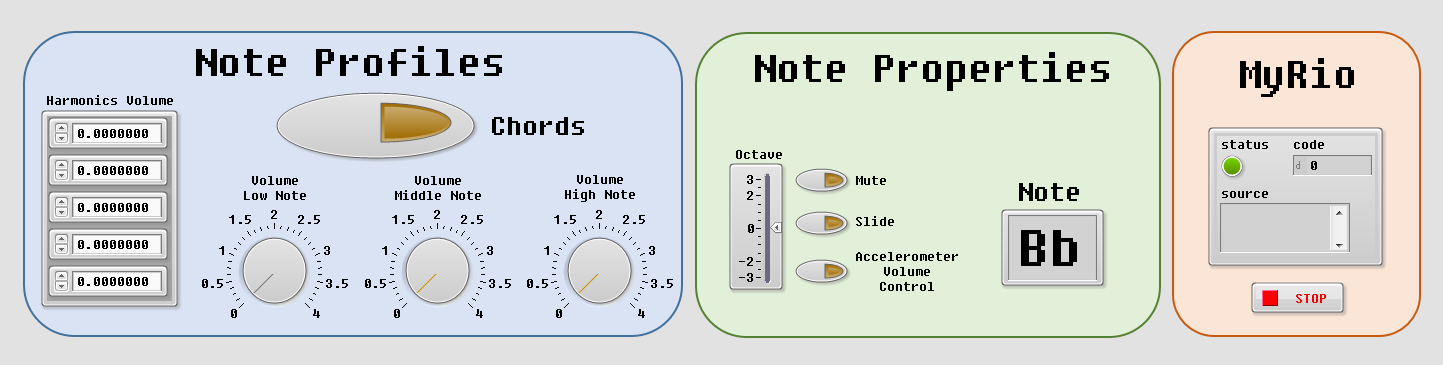
\includegraphics[width=3.5in]{instrumentfrontpanel.png}
\DeclareGraphicsExtensions.
\caption{Front panel for user input of the custom musical instrument.}
\label{fig_p1front}
\end{figure} 

\begin{figure}[!t]
\centering
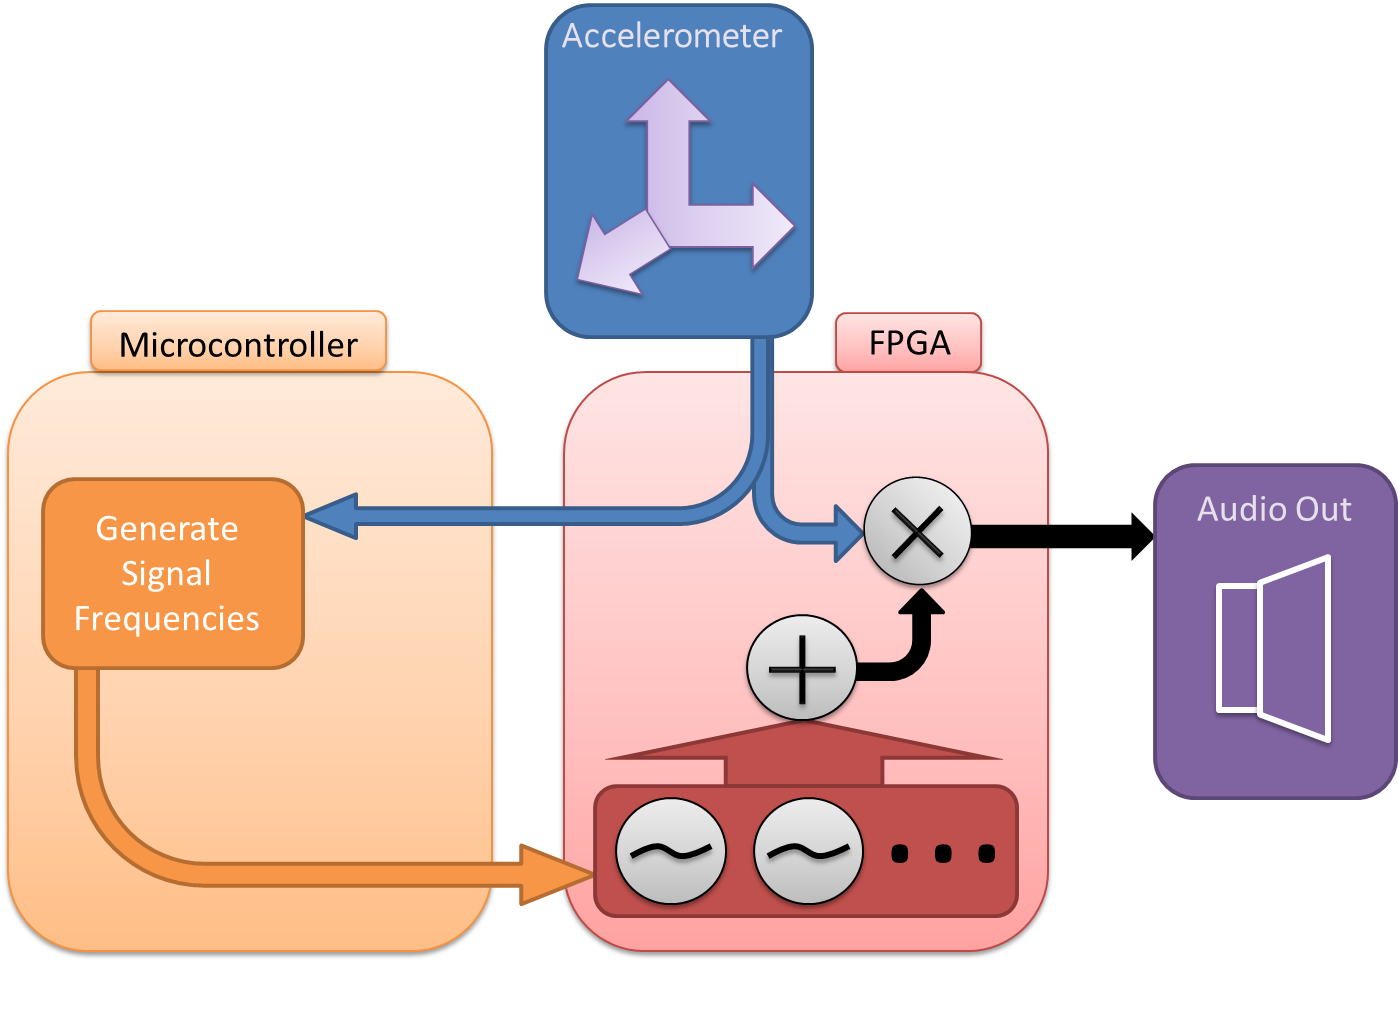
\includegraphics[width=3in]{part1blockdiagram.png}
\DeclareGraphicsExtensions.
\caption{Block diagram of the implementaion of the musical instrument.}
\label{fig_p1block}
\end{figure} 

\subsection{Frequency Generation}

When generating the fundamental frequencies on the microprocessor, a button is used to control whether the board will be outputting chords or single notes (Chords), and a button used to control whether the notes being output are continuous or discrete (Slide).
 If the Slide button is pressed, we simply take the y-component of the accelerometer and manipulate it using arithmetic operations and send that frequency to be adjusted by the Octave slide on the front panel, to be discussed later.
 Alternatively, if the Slide button is not pressed, the y-component of the acceleration is sent to a custom made VI which discretizes the frequency into discrete notes.

This custom VI takes in the y-acceleration as input and outputs the discrete frequency representing a particular note and a string letter representation of the output frequency.
 The output frequency will be 1 of 11 notes of a pentatonic scale with the blues note added spanning over two octaves (\(B_{2} - D_{3} - E_{3} - G_{3} - A_{3} - B^{b}_{3} - B_{3} - D_{4} - E_{4} - G_{4} - A_{4}\)) and is calculated using a sum of step functions.
 In order to obtain the frequency of a respective note, the entire range of accelerometer values is first divided into 12 ranges, where each range is assigned to a particular note.
 The input accelerometer values is subtracted by the upper limits of these ranges and the values will be used to shift the step functions of each note.
 Since the step functions now output values of 0 or 1 depending on the value of the accelerometer input, then if the accelerometer value is within a certain range, all step functions below and including the current range will output 1, while the ones connected to the higher notes will output 0.
 The value of the first note is directly multiplied by the value of its step function, but for subsequent notes, the difference between the frequencies of the current note and the previous note is multiplied by the value of its step function.
 The outputs of the step functions are finally added together and we obtain an equation for the discrete notes, seen below.
\begin{equation}
\label{hargen}
\begin{split}
 f_{dis}=f_{0}\cdot u \left( t- \left( A_{y}- \left( 260- \left( n-1  \right) \cdot \frac{520}{n} \right) \right) \right) +\\ \sum_{i=1, j=2}^{i=11,j=n-1}\Delta f_{i-1,i} \cdot u\left (t-\left (A_{y}-\left (260- \left( n-1  \right) \cdot \frac{520}{n}  \right) \right) \right)
\end{split}
\end{equation}

In equation \ref{hargen}, $i$ represents the indexed frequencies of musical notes, $j$ represents the index of the accelerometer ranges, and $n = 12$ represents the number of accelerometer ranges.

The string representation of the output frequency is obtained by retrieving a certain index in a pre-defined string array.
 This index is obtained by adding the values of each of the step functions.

An Octave slide is used to increase and decrease the octave of either the continuous or discrete notes.
 This is done using a scale by power of 2 function, since going up or down an octave is done by simply multiplying/dividing the frequency by 2.

Power chords were then generated by adding a note with its fifth, which is 1.5 times the the notes fundamental frequency \cite{power_chords}.
 The next octave (2x) of the note is also added in order to increase the fullness of the sound.
 Finally, the calculated fundamental frequencies are used to generate audio signals in the FPGA.

\subsection{Signal Generation and Processing}
The instrument creates a tone quality for each note by generating the fundamental frequency signal and combining it with the four subsequent harmonics.
 Since the operations required for signal generation and processing require fast performance, the signal generation and processing logic is designed on the onboard FPGA of the NI myRIO \cite{rt_comparison}.
 Fig. \ref{fig_notegen} shows the implementation of signal generation in LabVIEW.
 Sine wave generator blocks are used to produce a sine wave at a calculated frequency and a set sampling rate of 44 kHz, chosen due to its common usage for audio sampling \cite{sampling_rate}.
 To produce four subsequent harmonics, the calculated frequency is multiplied by integer factors, two through five, and the resultant frequencies are used as input to separate sine wave generator blocks.
 An array of fixed point numbers contain the gain level of each harmonic are converted into a cluster, de-bundled, and then multiplied to the output of their respective sine waves before they are summed together.
 This allows for variable tone quality by changing the volume of each harmonic.
 Multiplication is carried out using fixed point arithmetic for increased precision, requiring the 16 bit integer outputs of the sine wave generator to be converted to fixed point.

Three instances of the signal generation code are used to generate three separate notes. 
Similar to the harmonic volume each note is multiplied by a fixed point number gain to control the volume of each note. 
Chords are implemented by a summation of the three separate notes.

Acceleration controlled volume level of the output signal is achieved through scaling the raw acceleration data from the native accelerometer to the myRIO, and multiplying the result with the output signal. 
Similar to signal generation, multiplication is carried out using fixed point numbers for precision. 
 Fig. \ref{fig_accvol} shows the implementation of signal volume control in LabVIEW.
 A select block controlled by a control is used to switch between the signal at acceleration controlled volume and at maximum volume.
 Mute functionality is implemented similarly with a select block switching between the generated signal and no signal.
 The onboard button is also used to toggle the mute control when pressed and held, achieved by a select block and a not gate in the microcontroller code.


\begin{figure}[!t]
\centering
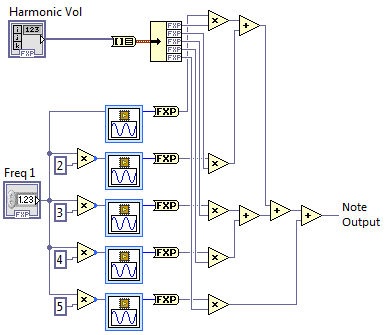
\includegraphics[width=3in]{NoteGeneration.png}
\DeclareGraphicsExtensions.
\caption{LabVIEW code for generating the summation of a sine wave and four of its harmonics.}
\label{fig_notegen}
\end{figure} 

\begin{figure}[!t]
\centering
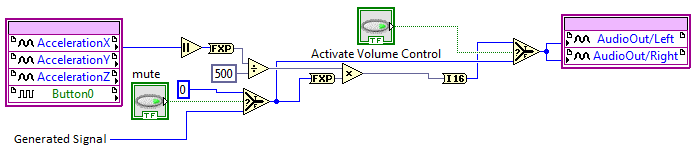
\includegraphics[width=3.5in]{AccelerometerVolume.png}
\DeclareGraphicsExtensions.
\caption{LabVIEW code for changing the gain on the output signal using accelerometer data and controls.}
\label{fig_accvol}
\end{figure} 



% needed in second column of first page if using \IEEEpubid
%\IEEEpubidadjcol

\section{Audio Effects Processing Unit}
The audio effects processing unit (AEPU) was required to have four functions: Left-right balance, 3-band equalization, echo, and master volume. 
These functions were implemented on a second myRIO board from the instrument.
The entirety of the signal processing was done on the FPGA with the microprocessor responsible for supplying varioius parameters, most from user input via the front panel in labView shown in Figure \ref{fig_AEPUfp}. 
It was chosen to have all of the singnal processing allocated to the FPGA to attempt to have the highest processing speed possible to maintain the best sound quality.
The FPGA was run at its maximum clock frequency of 40MHz, however the audio processing was done in a timed loop sampling at 20kHz, which is near maximum audible frequency for humans meaning the audio signal sound quality should be minimally affected. 
The overall block diagram of the system can be seen in Figure \ref{fig_AEPUBlock}.
As well, the implementation of the AEPU on the microprocessor can be found in Figure \ref{fig_AEPUMicro}.

\begin{figure}[!t]
\centering
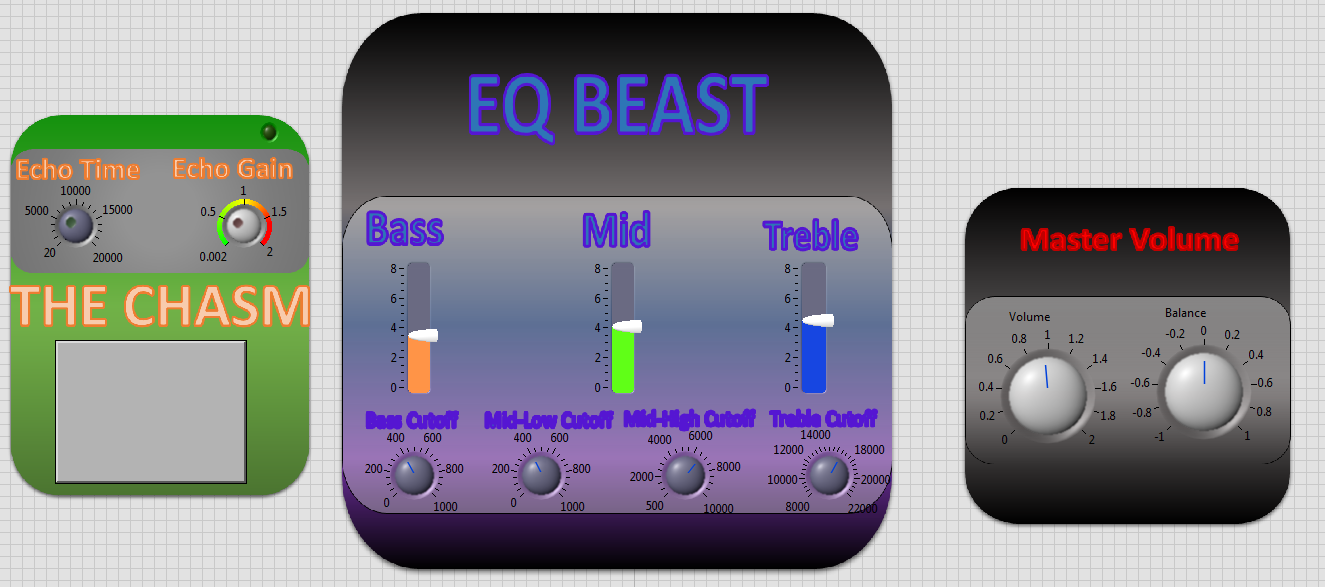
\includegraphics[width=3.3in]{frontpanel.png}
\DeclareGraphicsExtensions.
\caption{LabView front panel UI for the effects processing unit}
\label{fig_AEPUfp}
\end{figure}

\begin{figure}[!t]
\centering
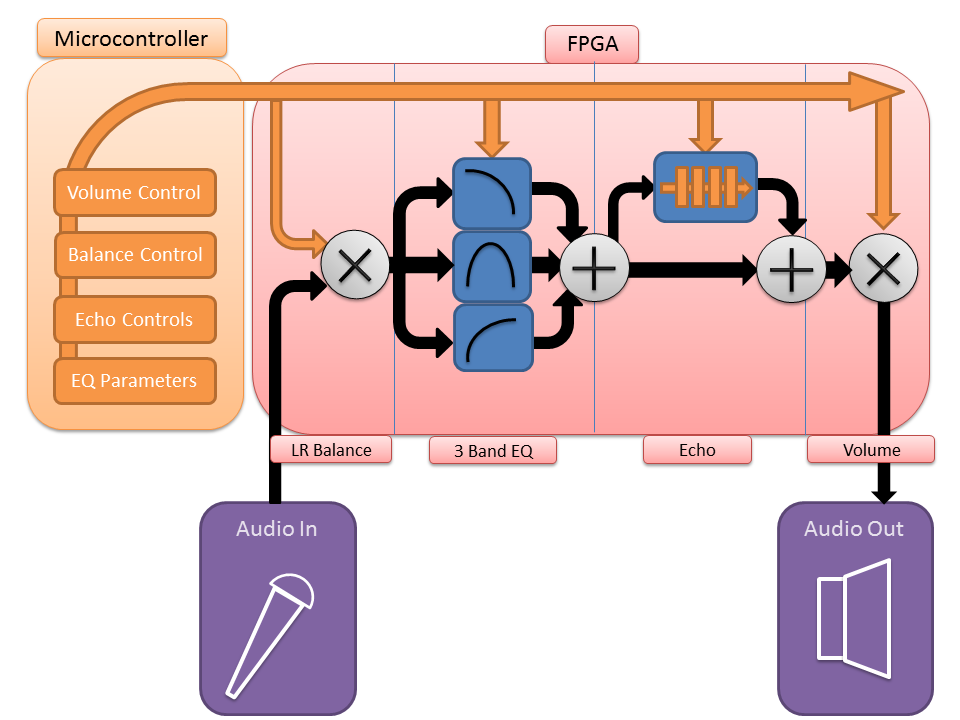
\includegraphics[width=3.3in]{aepublock.png}
\DeclareGraphicsExtensions.
\caption{Overall block diagram of the audio effects processing unit}
\label{fig_AEPUBlock}
\end{figure}



\subsection{Left-Right Balance}
The left-right balance effect which processes the audio signal on the FPGA unit, takes as input a fixed point value between -1 and 1 from the microprocessor obtained from the front panel control. 
The value passed in from the microprocessor, labeled Balance in Figure \ref{fig_BEQ}, is subtracted from 1 for the left channel and added to 1 for the right channel. 
The resulting values are multiplied by their corresponding audio signal paths to scale the signal accordingly. The result is that at -1, the right channel is completely cancelled and at 1, the left channel is completely canceled. 
The FPGA implemented block diagram can be seen on the left side of Figure \ref{fig_BEQ}.

\begin{figure}[!t]
\centering
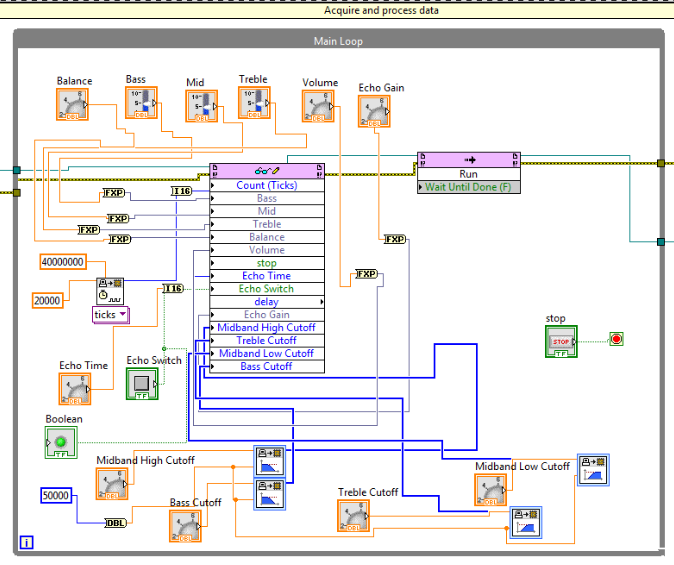
\includegraphics[width=3.3in]{microcontroller.png}
\DeclareGraphicsExtensions.
\caption{Microprocessor implementation of parameter-supplying interface}
\label{fig_AEPUMicro}
\end{figure}

\subsection{3-Band Equalizer}
The next step in the signal path was the 3-band equalizer, which can be seen in Figure \ref{fig_BEQ}. 
Each channel was fed into three parallel filters which were either low-pass or high-pass filters.
The cutoff frequency of each filter was controlled from the front panel of the microcontroller, where it was fed into a Butterworth Filter Coefficient subvi, and passed into the FPGA as a fixed point number.
As well, the gain for each band is taken from the front panel of the microcontroller, converted to fixed point, and fed into the FPGA.
The range of the coefficients is such that there can be slight overlap in the bands, while the range of the gain is from 0 to 8.
The bass-band filter was implemented as a low-pass filter, as was the upper-limit of the mid-band.
The lower-limit of the mid-band and the treble were implemented as high-pass filters.
By using both a low-pass and a high-pass filter for the mid-range band, the combined effect is a band-pass filter.
After each filter, the signals are converted back to 16-bit integers.
At the end of the equalizer stage. the split-signals of each channel are recombined into one and fed into the echo stage.

\begin{figure}[!t]
\centering
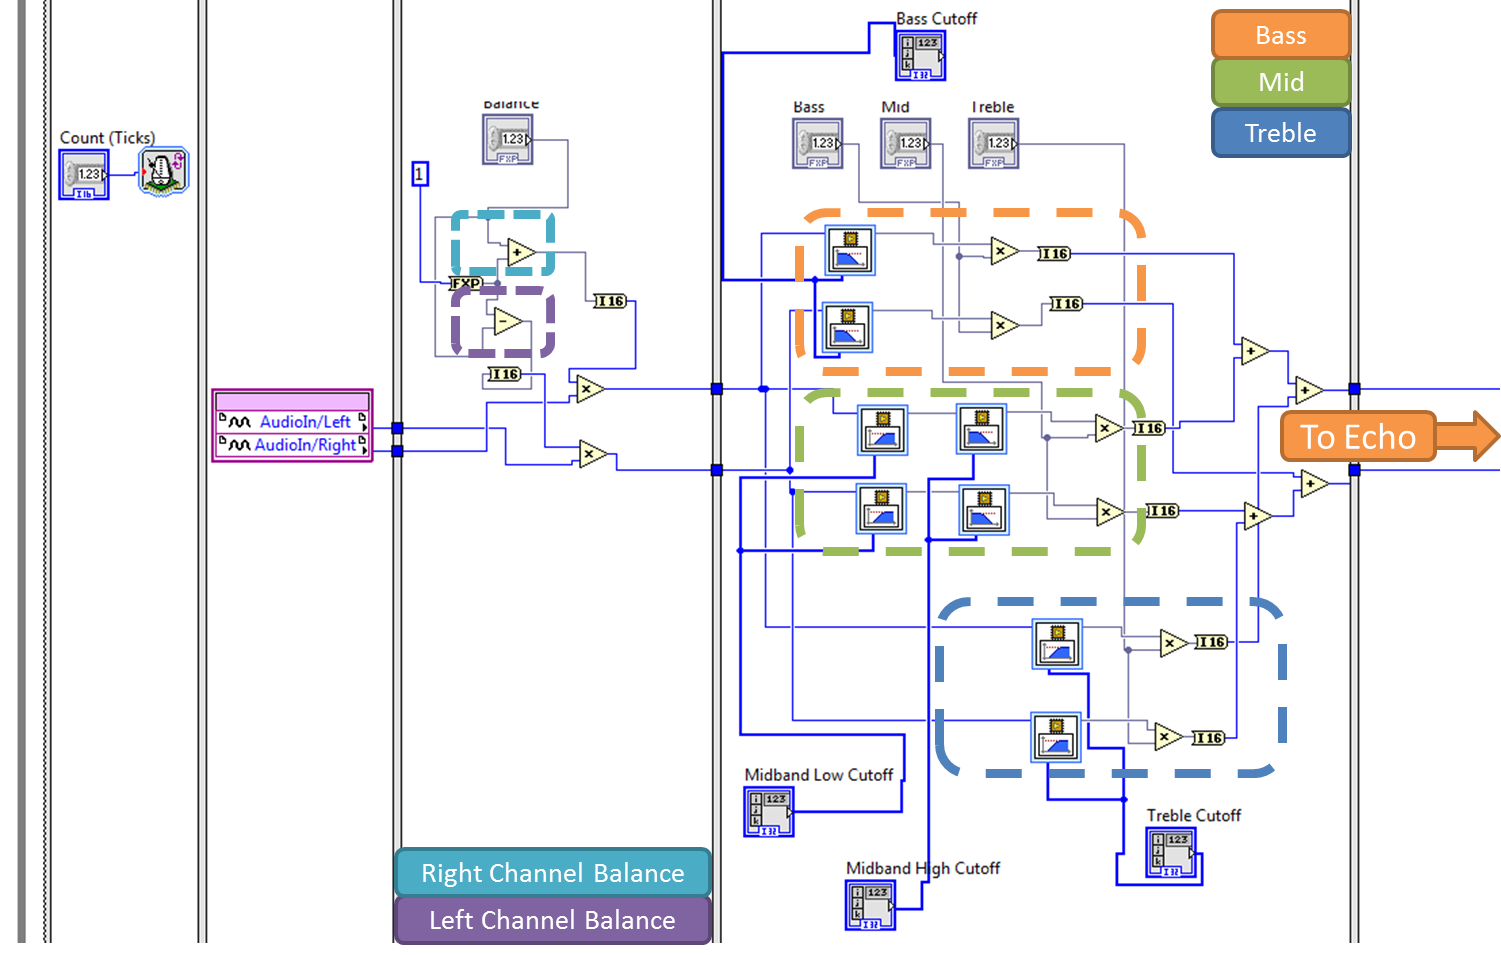
\includegraphics[width=3.3in]{balanceandeq.png}
\DeclareGraphicsExtensions.
\caption{labVIEW FPGA implementation of left-right balance and 3-band equalizer}
\label{fig_BEQ}
\end{figure}  

\subsection{Echo}
Echo is implemented in entirely in the FPGA with the parameters Echo Time and Echo Gain passed to the FPGA from the microcontroller in the same fashion as the previously described functions. 
The corresponding FPGA implemented block diagram can be seen in Figure \ref{fig_echo}.
To echo the signal, the samples must be written to memory and read a specific time later (the echo time) to be combined with the main signal path. 
The memory was implemented using a FIFO queue for each audio channel. The FPGA resources on the myRIO only allowed for a maximum of 31000 elements on each FIFO which set the upper limit on the delay time. 
The time was implemented using a counter initialized at 0. Each loop iteration the counter increments by 1 until the Echo Time is reached. 
When the echo time is reached, the counter is no longer incremented and the echo time is continuously passed to the shift register to ensure that the counter remains equal to the echo time.
If the echo time is increased, the counter begins incrementing again. If the echo time is decreased below the counter value, the counter is reset to 0 and the FIFOs are cleared. 
Whenever the counter is equal to the echo time, the case structure is set to true which reads a sample every loop iteration. 
When the counter is not equal to the echo time, 0 is combined with the current signal. 
A fixed point value between 0 and 2 labelled Echo Gain in Figure \ref{fig_echo} is also passed from the microprocessor and is multiplied by the echo signal before it is added back into the main signal path. 
This allows for either an attenuation of amplification of the echoed signal depending on user preferences.  

\begin{figure}[!t]
\centering
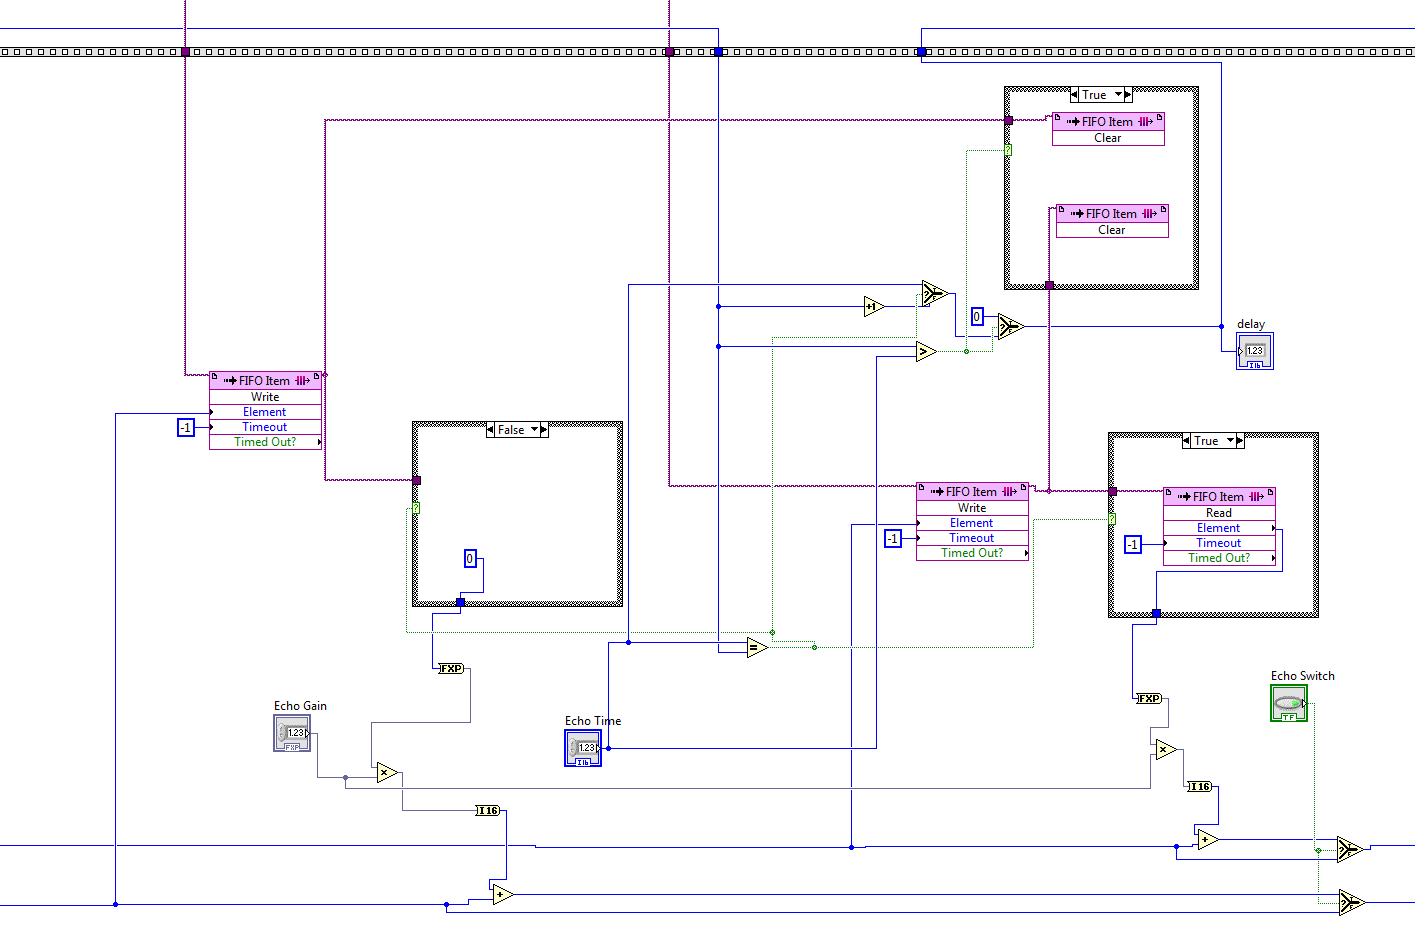
\includegraphics[width=3.5in]{echo.png}
\DeclareGraphicsExtensions.
\caption{labVIEW FPGA implementation of echo}
\label{fig_echo}
\end{figure} 

\begin{figure}[!t]
\centering
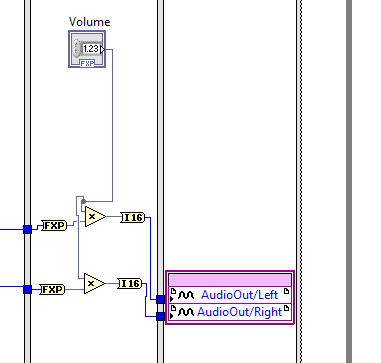
\includegraphics[width=2.5in]{volume.png}
\DeclareGraphicsExtensions.
\caption{labVIEW FPGA implementation of volume control}
\label{fig_volume}
\end{figure} 

\subsection{Master Volume}

The last step in the signal path of the AEPU was the master volume control shown in Figure \ref{fig_volume}.
Its implementation was straightforward: a double was selected from the front-panel of the microcontroller between 0 and 2, converted to fixed point, and fed into the FPGA.
Then, it was multpilied by the signal of both the left and right channel and converted back into a 16-bit integer.
This results in either a gain or attenuation depending on what value was chosen.

% An example of a floating figure using the graphicx package.
% Note that \label must occur AFTER (or within) \caption.
% For figures, \caption should occur after the \includegraphics.
% Note that IEEEtran v1.7 and later has special internal code that
% is designed to preserve the operation of \label within \caption
% even when the captionsoff option is in effect. However, because
% of issues like this, it may be the safest practice to put all your
% \label just after \caption rather than within \caption{}.
%
% Reminder: the "draftcls" or "draftclsnofoot", not "draft", class
% option should be used if it is desired that the figures are to be
% displayed while in draft mode.
%
%\begin{figure}[!t]
%\centering
%\includegraphics[width=2.5in]{myfigure}
% where an .eps filename suffix will be assumed under latex,
% and a .pdf suffix will be assumed for pdflatex; or what has been declared
% via \DeclareGraphicsExtensions.
%\caption{Simulation Results}
%\label{fig_mimodiag}
%\end{figure}

% Note that IEEE typically puts floats only at the top, even when this
% results in a large percentage of a column being occupied by floats.


% An example of a double column floating figure using two subfigures.
% (The subfig.sty package must be loaded for this to work.)
% The subfigure \label commands are set within each subfloat command, the
% \label for the overall figure must come after \caption.
% \hfil must be used as a separator to get equal spacing.
% The subfigure.sty package works much the same way, except \subfigure is
% used instead of \subfloat.
%
%\begin{figure*}[!t]
%\centerline{\subfloat[Case I]\includegraphics[width=2.5in]{subfigcase1}%
%\label{fig_first_case}}
%\hfil
%\subfloat[Case II]{\includegraphics[width=2.5in]{subfigcase2}%
%\label{fig_second_case}}}
%\caption{Simulation results}
%\label{fig_sim}
%\end{figure*}
%
% Note that often IEEE papers with subfigures do not employ subfigure
% captions (using the optional argument to \subfloat), but instead will
% reference/describe all of them (a), (b), etc., within the main caption.


% An example of a floating table. Note that, for IEEE style tables, the
% \caption command should come BEFORE the table. Table text will default to
% \footnotesize as IEEE normally uses this smaller font for tables.
% The \label must come after \caption as always.
%
%\begin{table}[!t]
%% increase table row spacing, adjust to taste
%\renewcommand{\arraystretch}{1.3}
% if using array.sty, it might be a good idea to tweak the value of
% \extrarowheight as needed to properly center the text within the cells
%\caption{An Example of a Table}
%\label{table_example}
%\centering
%% Some packages, such as MDW tools, offer better commands for making tables
%% than the plain LaTeX2e tabular which is used here.
%\begin{tabular}{|c||c|}
%\hline
%One & Two\\
%\hline
%Three & Four\\
%\hline
%\end{tabular}
%\end{table}


% Note that IEEE does not put floats in the very first column - or typically
% anywhere on the first page for that matter. Also, in-text middle ("here")
% positioning is not used. Most IEEE journals use top floats exclusively.
% Note that, LaTeX2e, unlike IEEE journals, places footnotes above bottom
% floats. This can be corrected via the \fnbelowfloat command of the
% stfloats package.



\section{Discussion}
\subsection{Custom Instrument}
The musical instrument unit was developed creating a basic instrument first and then adding features on using a modular approach. 
 Initially implementing a basic sound generator was essential since testing required listening to the changes in the sounds produced by the instrument.

To test generating frequencies the board wad moved in the y-direction and the 11 discrete notes were compared to tones generated by a known source. The non-discretized pitch control was tested by listening for a continuous pitch change along the entire range of the accelerometer values. Chords were tested by differentiating between three different notes being played simultaneously using their seperate volume controls. Octave changes were tested by listening to the note and making sure that the pitch increased but the note remained constant.

Volume control using the accelerometer was first implemented by multiplying the output audio signal with the 16 bit integer value of the acceleration in the x-direction.
 The volume range was too large for stable control by the user, therefore fixed point conversion and scaling the raw acceleration data before multiplication with the output signal was implemented.
 A scaling factor of 50 was chosen since it produced an optimal volume range.

Tone quality was the final implemented feature to maximize FPGA usage.
 More sine wave generator blocks per note lead to a wider range of sounds; however, these blocks require a large amount of FPGA resources in LUTs.
 The optimal amount of signal generators was chosen through trial and error to be five per note, (resulting in fifteen in total for the entire FPGA), using 82% of the LUTs available.
 Adding more sine wave generator blocks result in an overuse of resources despite there being 18% of LUTs remaining, most likely due to routing constraints.

\subsection{Audio Effects Processing Unit}
The audio effects processing unit was developed one component at a time, working up from what was estimated as the easiest implementation to the most difficult. 
Volume and left-right balance were first to be implemented and little trouble was had in their development. Some adjustments were made later on regarding the amount of maximum gain to allow each stage to prevent distortion in the final output signal. 
3-band equalization was next to be implemented and was also not much trouble as the filter VIs in LabView are very intuitive to use.
 Again there was some adjustments made regarding gain later on in development, as well as the addition of tunable filter range as an extra feature. 
The most difficult of the functions was echo. 
The first attempt consisted of using a large array (30000 elements) which would be used to store samples. 
The echoed sample would then be pulled out of the array a designated number of elements from the front of the array. Unfortunately, even an array of 100 elements was enough to maximize the resources of the FPGA. 
Replacing the array with a FIFO queue alleviated this problem, and a counter was implemented to replace the index selection of the array method. 
This worked, however due to a timeout issue with the FIFO queues, the echo time was fixed at approximately 2 seconds until the an attempt was made to override the timeout, which fixed the issue. 
Finally, when the echo time was reduced below the current value of the counter, some issue with the FIFO was causing the FPGA to crash completely where it would then need to be rebooted. 
This issue was probably attributed to the FIFO queues reaching maximum capacity before a sample was read. 
This issue was fixed by clearing the FIFO every time this event occurred. 


\section{Conclusion}
The result of this project was a musical instrument that has a robust amount of features and is fun to play.
 In hindsight, to reduce time spent on FPGA compilations, it would have been beneficial to fully design the FPGA code before implementation instead of an iteratively adding to the code.
 Also, indicators and waveform charts were an indispensable resource for debugging the code.
 Furthermore, other features such as vibrato, playback, and accelerometer stabilization were discussed but scrapped due to time constraints.

% if have a single appendix:
%\appendix[Proof of the Zonklar Equations]
% or
%\appendix  % for no appendix heading
% do not use \section anymore after \appendix, only \section*
% is possibly needed

% use appendices with more than one appendix
% then use \section to start each appendix
% you must declare a \section before using any
% \subsection or using \label (\appendices by itself
% starts a section numbered zero.)
%





% use section* for acknowledgement
\section*{Acknowledgment}

Thank you to the teaching assistant Michael Yuhas whose help was invaluable throughout this development process and to Prof. Meyer for the opportunity to work on such an engaging project.

% trigger a \newpage just before the given reference
% number - used to balance the columns on the last page
% adjust value as needed - may need to be readjusted if
% the document is modified later
%\IEEEtriggeratref{8}
% The "triggered" command can be changed if desired:
%\IEEEtriggercmd{\enlargethispage{-5in}}

% references section

% can use a bibliography generated by BibTeX as a .bbl file
% BibTeX documentation can be easily obtained at:
% http://www.ctan.org/tex-archive/biblio/bibtex/contrib/doc/
% The IEEEtran BibTeX style support page is at:
% http://www.michaelshell.org/tex/ieeetran/bibtex/
\bibliographystyle{ieeetran}
% argument is your BibTeX string definitions and bibliography database(s)
\bibliography{references}
%
% <OR> manually copy in the resultant .bbl file
% set second argument of \begin to the number of references
% (used to reserve space for the reference number labels box)


% biography section


\end{document}



